\documentclass{beamer}
\usepackage[utf8]{inputenc}

\usetheme{Madrid}
\usecolortheme{default}
\usepackage{amsmath,amssymb,amsfonts,amsthm}
\usepackage{txfonts}
\usepackage{tkz-euclide}
\usepackage{listings}
\usepackage{adjustbox}
\usepackage{array}
\usepackage{tabularx}
\usepackage{gvv}
\usepackage{lmodern}
\usepackage{circuitikz}
\usepackage{tikz}
\usepackage{graphicx}

\setbeamertemplate{page number in head/foot}[totalframenumber]

\usepackage{tcolorbox}
\tcbuselibrary{minted,breakable,xparse,skins}



\definecolor{bg}{gray}{0.95}
\DeclareTCBListing{mintedbox}{O{}m!O{}}{%
	breakable=true,
	listing engine=minted,
	listing only,
	minted language=#2,
	minted style=default,
	minted options={%
		linenos,
		gobble=0,
		breaklines=true,
		breakafter=,,
		fontsize=\small,
		numbersep=8pt,
		#1},
	boxsep=0pt,
	left skip=0pt,
	right skip=0pt,
	left=25pt,
	right=0pt,
	top=3pt,
	bottom=3pt,
	arc=5pt,
	leftrule=0pt,
	rightrule=0pt,
	bottomrule=2pt,
	toprule=2pt,
	colback=bg,
	colframe=orange!70,
	enhanced,
	overlay={%
		\begin{tcbclipinterior}
			\fill[orange!20!white] (frame.south west) rectangle ([xshift=20pt]frame.north west);
	\end{tcbclipinterior}},
	#3,
}
\lstset{
	language=C,
	basicstyle=\ttfamily\small,
	keywordstyle=\color{blue},
	stringstyle=\color{orange},
	commentstyle=\color{green!60!black},
	numbers=left,
	numberstyle=\tiny\color{gray},
	breaklines=true,
	showstringspaces=false,
}
\begin{document}

\title 
{2.10.69}
\date{10 September,2025}

\author 
{Naman Kumar-EE25BTECH11041}
\graphicspath{./figs}


\frame{\titlepage}
\begin{frame}{Question}
Determine the value of c so that for all real x, the vector $cx\hat{\imath}-6\hat{\jmath}-3\hat{k}$ and $x\hat{\imath}+2\hat{\jmath}+2cx\hat{k}$ make an obtuse angle with each other.
\end{frame}
\begin{frame}{Solution}
    We know, Inner product of two vectors
\begin{align}
    \vec{A}^T\vec{B}=\lVert\vec{A}\rVert\lVert\vec{B}\rVert \cos{\theta}
\end{align}
for obtuse angle between any two vectors
\begin{align}
\cos{\theta}<0\text{ or } \vec{A}^T\vec{B}<0
\end{align}
Given Vectors
\begin{align}
    \vec{A}=\begin{pmatrix}cx\\-6\\-3\end{pmatrix},
    \vec{b}=\begin{pmatrix}x\\2\\2cx\end{pmatrix}
\end{align}
\end{frame}
\begin{frame}{Solution}
Now using these condition on given vectors
\begin{align}
\vec{A}^T\vec{B}<0\\
\begin{pmatrix}cx&-6&-3\end{pmatrix}\begin{pmatrix}x\\2\\2cx\end{pmatrix}<0\\
cx^2-12-6cx<0\text{ ( quadratic in x)} \label{quad}
\end{align}
for any quadratic to be negative $\forall x \in R$, their are two conditions
\begin{align}
    a<0 \&D<0\\
\end{align}
\end{frame}
\begin{frame}{Solution}
Now applying this conditions on \eqref{quad}
firstly on a (leading coefficient)
\begin{align}
    c<0 \label{1}
\end{align}
on D (discriminant)
\begin{align}
    D=b^2-4ac<0\\
    (-6c)^2-4\times c \times(-12)<0\\
    36c^2+48c<0\\
    c(3c+4)<0 \label{2}
\end{align}
therfore, by taking union of \eqref{1} and \eqref{2} 
\begin{align}
    c\in(\frac{-4}{3}, 0)
\end{align}
\end{frame}
\begin{frame}{Figure}
    \begin{figure}[H]
    \centering
    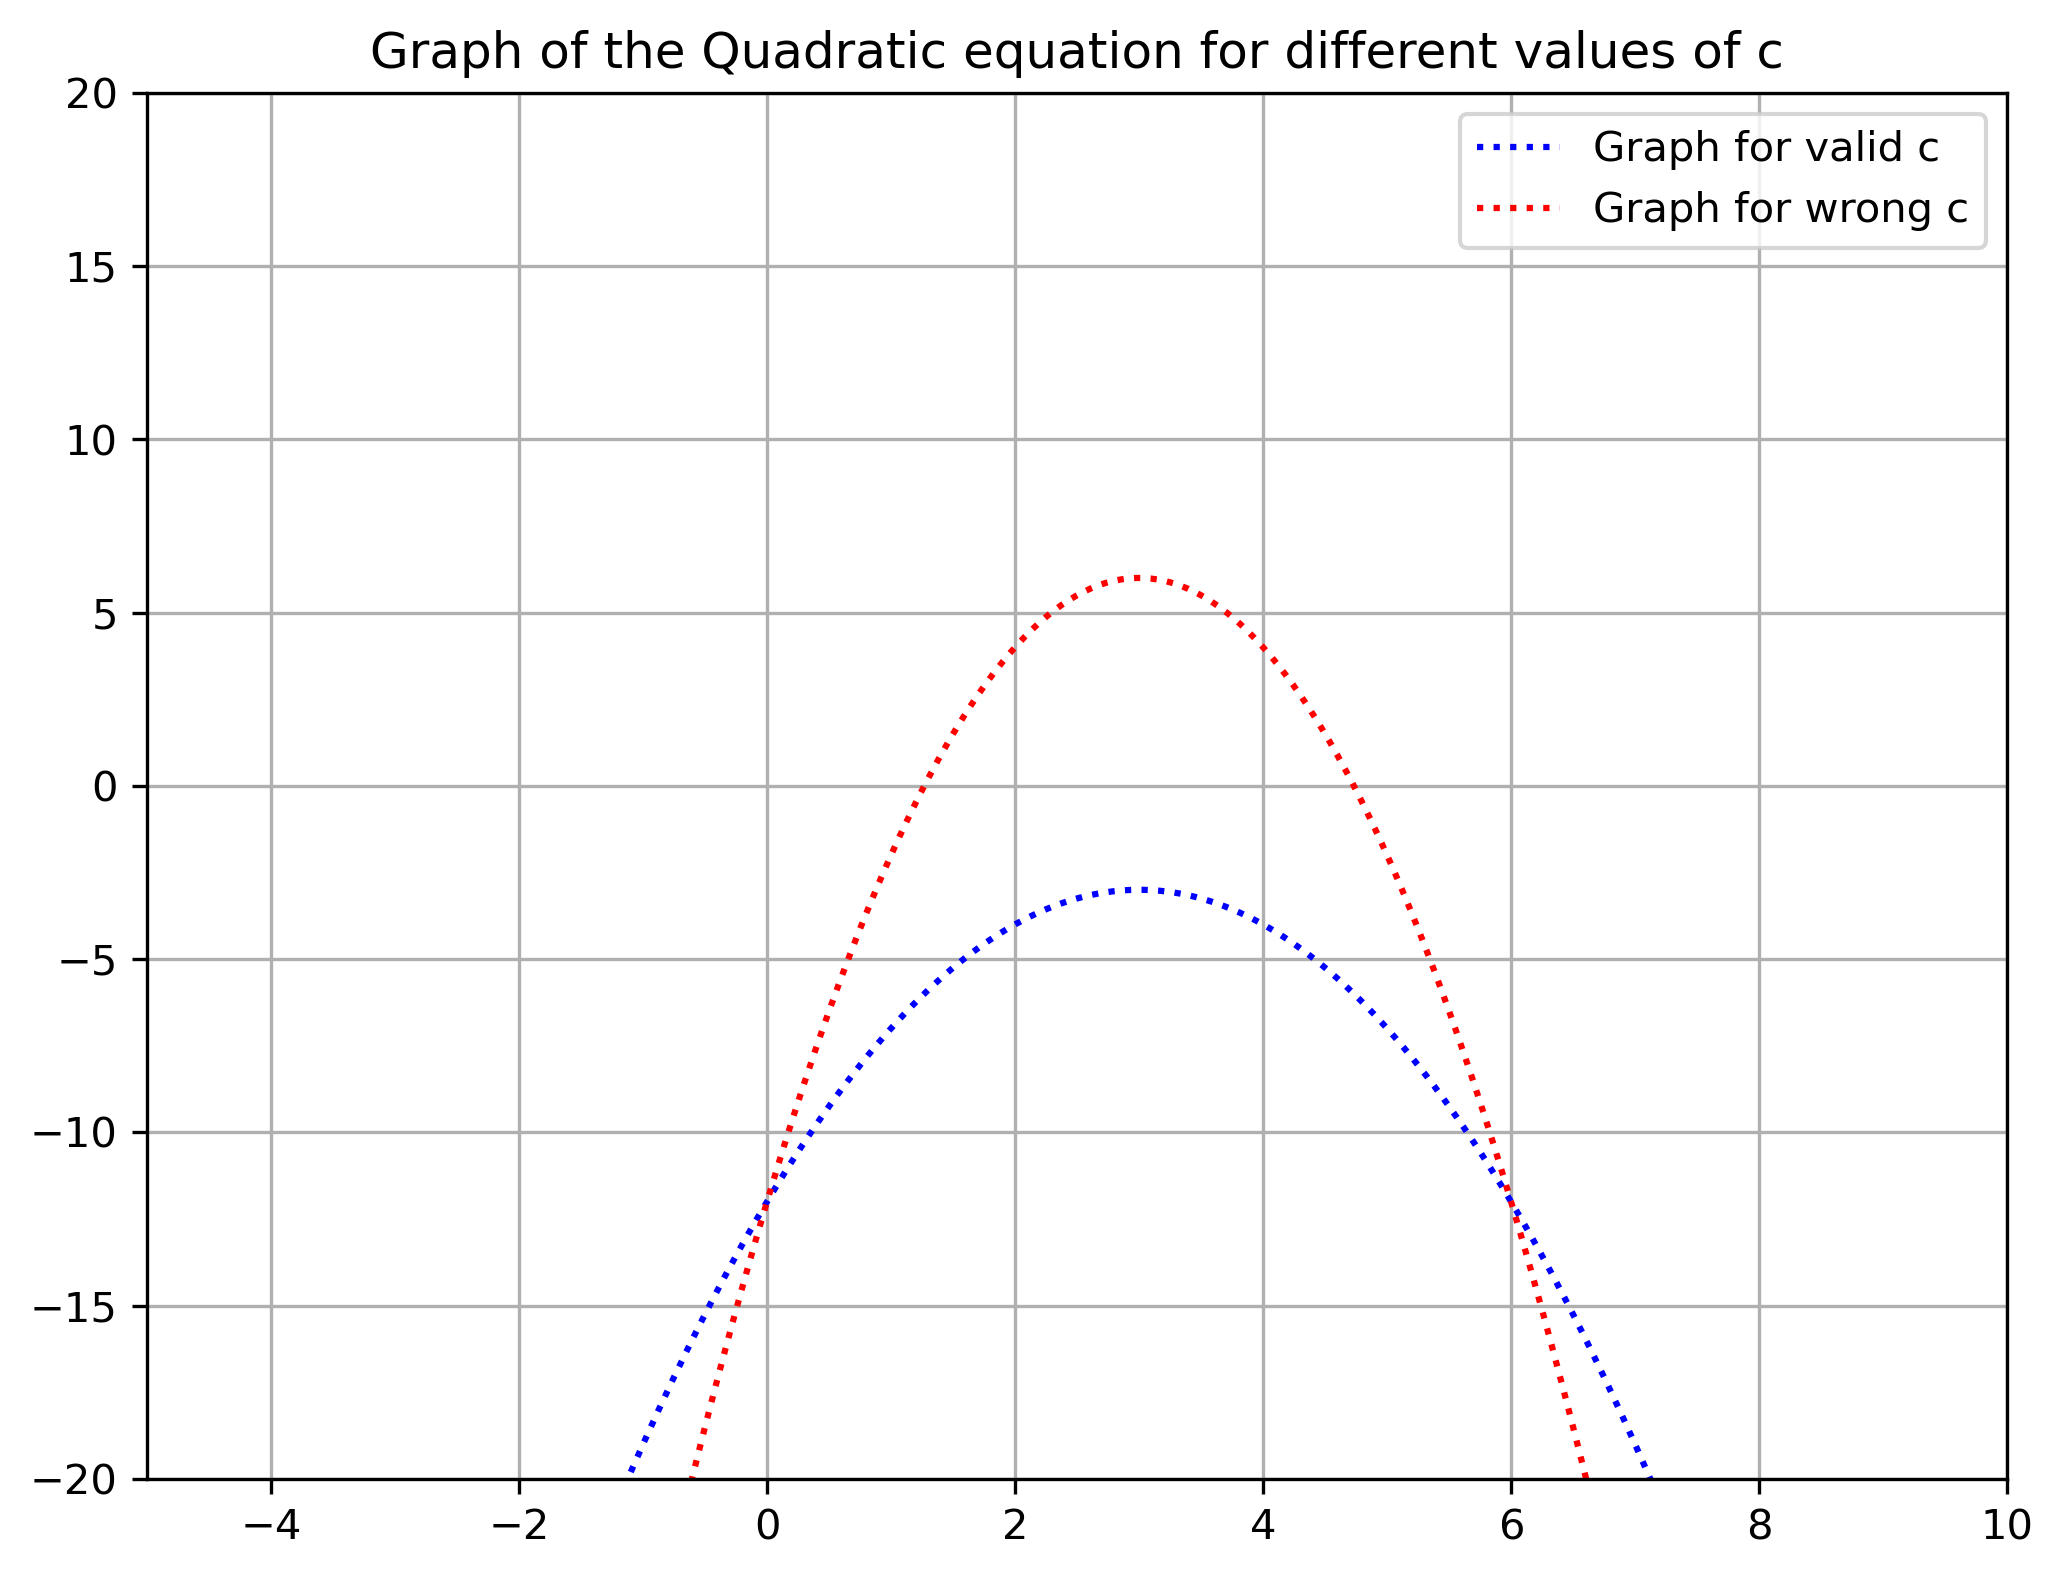
\includegraphics[width=0.6\columnwidth]{figs/figure.png}
    \label{fig:placeholder}
\end{figure}
\end{frame}

\begin{frame}[fragile]
\frametitle{C code}
\begin{lstlisting}
#include <stdio.h>
#include <math.h>

void dot_product(double vector1[], double vector2[], int size, double* result) {
    *result = 0.0;
    for (int i = 0; i < size; i++) {
        *result += vector1[i] * vector2[i];
    }
}
\end{lstlisting}
\end{frame}
\begin{frame}[fragile]
\frametitle{Direct python code}
\begin{lstlisting}
import numpy as np
import matplotlib.pyplot as plt

plt.figure(figsize=(8, 6), dpi=100)  

def quad(c,x):
    return c*x**2-6*c*x-12


x=np.linspace(-15,15,500)
c_valid=-1
y = quad(c_valid, x)
plt.plot(x,y, ':b', label="Graph for valid c")
\end{lstlisting}
\end{frame}
\begin{frame}[fragile]
\frametitle{Direct python code}
\begin{lstlisting}
x=np.linspace(-15,15,500)
c_wrong=-2
y=quad(c_wrong, x)
plt.plot(x,y, ':r', label="Graph for wrong c")

plt.legend()
plt.grid()
plt.xlim(-5, 10)
plt.ylim(-20, 20)
plt.savefig('figure.png', dpi=300, bbox_inches='tight')
plt.show()
\end{lstlisting}
\end{frame}



\end{document}